% !TEX root = handbook-physics.tex
%!TEX TS-program = pdflatex
%!TEX encoding = UTF-8 Unicode

\chapter{Electric Charges. Coulomb's Law}
\label{ch-14}
\zhtitle{电荷。库仑定律}

\section{Introduction}
\label{sec-14.1}
\zhtitle{引言}

\subsection{}\label{14.1.1} \redem{Electrostatics} is the branch of the study of electricity that deals with the interaction and properties of a system of electric charges that are fixed with respect to the chosen inertial frame of reference \ssect{2.1.2}.
\zhpar{\redem{静电学}是电学的一个分支，研究相对于所选惯性参考系（\ssect{2.1.2}）固定不动的电荷系统的相互作用及其性质。}

There are two kinds of electric charges, \redem{positive} and \redem{negative}. Bodies having unlike charges attract one another; those having like charges repulse one another.
\zhpar{电荷有两种，即\redem{正}电荷和\redem{负}电荷。电荷异号的物体相互吸引，电荷同号的物体相互排斥。}

\subsection{}\label{14.1.2} The electric charge of any system of bodies consists of a whole number of elementary charges, each equal to \SI{1.6d-19}{\coulomb} (where C is the abbreviation of coulomb, the unit of charge). The stable particle with the minimum rest mass \ssect{5.6.1} and a negative elementary charge is the \redem{electron}. The rest mass of the electron is \SI{9.1d-31}{\kilo\gram}. The stable particle with the minimum rest mass and a positive elementary charge is the \redem{positron} \ssect{43.5.1}.\sidenote{Here we do not consider the instability of the positron, common in our world, that is associated with the annihilation of an electron-positron pair \ssect{43.5.1}.} Its rest mass is the same as that of the electron. Besides, there is a stable particle with a positive elementary charge called the \redem{proton}. The rest mass of the proton is \SI{1.67d-27}{\kilo\gram}. Electrons and protons are found in the atoms of all the chemical elements.
\zhpar{任何物体系统的电荷都由整数个基本电荷组成，每个基本电荷等于 \SI{1.6d-19}{\coulomb}（其中 C 为库仑的缩写，库仑是电荷的单位）。静止质量最小（\ssect{5.6.1}）且带负基本电荷的稳定粒子是\redem{电子}，其静止质量为 \SI{9.1d-31}{\kilo\gram}。静止质量最小且带正基本电荷的稳定粒子是\redem{正电子}（\ssect{43.5.1}），其静止质量与电子相同。此外，还有一种带正基本电荷的稳定粒子，称为\redem{质子}，其静止质量为 \SI{1.67d-27}{\kilo\gram}。电子和质子存在于所有化学元素的原子中。}
\zhpar{注：此处不考虑正电子的不稳定性。正电子的不稳定性在我们的世界中很常见，与电子-正电子对的湮灭有关（见\ssect{43.5.1}）。}

\subsection{}\label{14.1.3} The \redem{law of conservation of electric charge} states: the algebraic sum of the electric charges of bodies or particles that constitute an electrically isolated system remains constant re­ gardless of any processes that occur in the system.
\zhpar{\redem{电荷守恒定律}指出：构成电隔离系统的物体或粒子所带电荷的代数和，与系统内发生的任何过程无关，始终保持不变。}

New electrically charged particles may be formed in the system being considered. These may be electrons formed by the ionization of atoms or molecules \ssect{22.4.1}, ions formed by the phenomenon of electrolytic dissociation, etc. If the system is electrically isolated, however, then the algebraic sum of the charges of all the newly formed particles of the system always equals zero. The law of the conservation of electric charge is one of the fundamental conservation laws, like the laws of conservation of momentum \ssect{2.7.1} and of energy \ssect{3.4.2}.
\zhpar{在所考虑的系统中，可能会形成新的带电粒子，例如原子或分子电离时形成的电子（\ssect{22.4.1}），以及电解离过程形成的离子等。但若系统是电隔离的，则系统内所有新形成粒子的电荷代数和始终为零。电荷守恒定律与动量守恒定律（\ssect{2.7.1}）和能量守恒定律（\ssect{3.4.2}）一样，是基本守恒定律之一。}

\subsection{}\label{14.1.4} Upon contact of two electrically neutral bodies, charges go over from one body to the other as a result of friction. In each of such two bodies there is no longer an equal number of positive and negative charges and the bodies become oppositely charged.
\zhpar{两个电中性的物体接触时，由于摩擦，电荷会从一个物体转移到另一个物体。于是，这两个物体中正负电荷的数目不再相等，两个物体带上了符号相反的电荷。}

When a body is electrized by induction, the charges in it are no longer uniformly distributed. The charges are redistributed so that one part of the body has an excess of positive charges and the other part, of negative charges. If these two parts of the body are separated in some way, they will be oppositely charged.
\zhpar{物体通过感应起电时，其内部的电荷不再均匀分布。电荷重新分布，使物体的一部分带有多余的正电荷，另一部分带有多余的负电荷。若以某种方式将物体的这两部分分开，它们就会带上符号相反的电荷。}



\section{Coulomb's Law}
\label{sec-14.2}
\zhtitle{库仑定律}

\subsection{}\label{14.2.1} Coulomb experimentally established that the force of interaction $F_{12}$ between two small charged spheres, with charges equal to $q_{1}$ and $q_{2}$ \ssect{14.1.1}, is proportional to the product $q_{1}\,q_{2}$ and inversely proportional to the square of the distance $r$ between the spheres:
\zhpar{库仑通过实验确定：两个小带电球之间的相互作用力 $F_{12}$（两球电荷分别为 $q_{1}$ 和 $q_{2}$，见\ssect{14.1.1}），与电荷乘积 $q_{1}\,q_{2}$ 成正比，与两球之间距离 $r$ 的平方成反比，即：}
\begin{equation*}%
F_{12} = k_{1} \,\frac{q_{1}\,q_{2}}{r^{2}},
\end{equation*}
where $k_{1}$ is the proportionality factor $(k_{1} > 0)$.
\zhpar{式中 $k_{1}$ 为比例系数 $(k_{1} > 0)$。}

\subsection{}\label{14.2.2} \redem{Central forces} act on the charges along a straight line joining the centres of the charges. In the interaction of like charges the product $q_{1}q_{2} > 0$ and $F_{12} > 0$. This corresponds to mutual repulsion. For unlike charges $q_{1}q_{2} < 0$ and $F_{12} < 0$, which corresponds to mutual attraction. The vector form of the Coulomb law is
\zhpar{\redem{有心力}沿连接电荷中心的直线作用于电荷上。同号电荷相互作用时，$q_{1}q_{2} > 0$，$F_{12} > 0$，对应于相互排斥。异号电荷相互作用时，$q_{1}q_{2} < 0$，$F_{12} < 0$，对应于相互吸引。库仑定律的矢量形式为：}
\begin{equation*}%
\vb{F}_{12} = k_{1} \,\frac{q_{1}\,q_{2}}{r^{2}} \, \frac{\vb{r}_{12}}{r},
\end{equation*}
where $\vb{F}_{12}$ is the force exerted on charge $q_{1}$ by charge $q_{2}$, $\vb{r}_{12}$ is the radius vector joining charge $q_{2}$ to $q_{1}$ and $r = \abs{\vb{r}_{12}}$.
\zhpar{式中，$\vb{F}_{12}$ 是电荷 $q_{2}$ 作用于电荷 $q_{1}$ 上的力，$\vb{r}_{12}$ 是由电荷 $q_{2}$ 指向 $q_{1}$ 的位矢，$r = \abs{\vb{r}_{12}}$。}
\begin{marginfigure}
\centering
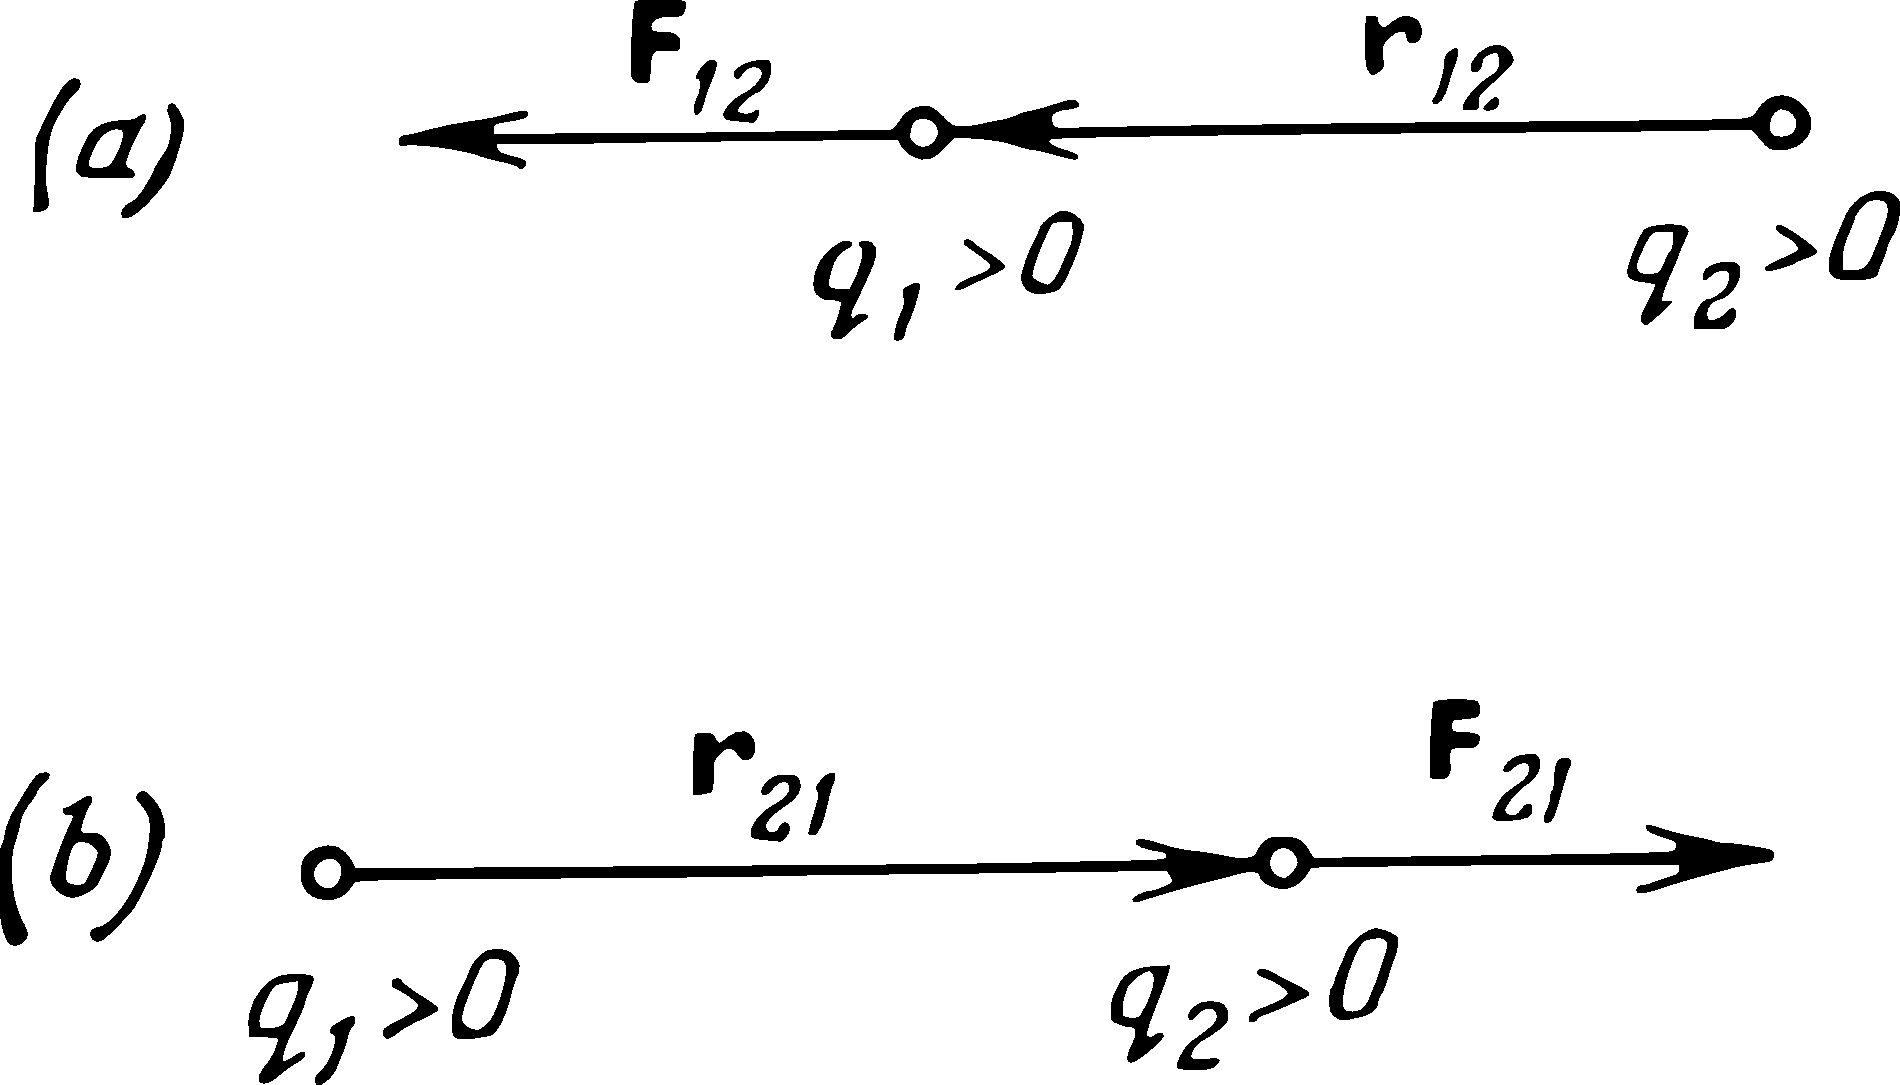
\includegraphics[width=0.8\textwidth]{figs/ch-14/fig-14-01.pdf}
\caption{Repulsive and attractive force between charges.\zhcap{电荷间的排斥力与吸引力。}\label{fig-14-01}}
\end{marginfigure}

The force $\vb{F}_{12}$, exerted on charge $q_{2}$ by charge $q_{1}$, equals
\zhpar{电荷 $q_{1}$ 作用于电荷 $q_{2}$ 上的力 $\vb{F}_{21}$ 为：}
\begin{equation*}%
\vb{F}_{12} = k_{1} \,\frac{q_{1}\,q_{2}}{r^{2}} \, \frac{\vb{r}_{12}}{r},
\end{equation*}
where $\vb{r}_{21} = - \vb{r}_{12}$ is the radius vector joining charges $q_{1}$ and $q_{2}$ (\figr{fig-14-01}~\inred{(b)}). Forces $\vb{F}_{12}$ and $\vb{F}_{21}$ are said to be \redem{Coulomb forces}. 
\zhpar{其中 $\vb{r}_{21} = - \vb{r}_{12}$ 是连接电荷 $q_{1}$ 和 $q_{2}$ 的位矢（见\figr{fig-14-01}~\inred{(b)}）。力 $\vb{F}_{12}$ 和 $\vb{F}_{21}$ 称为\redem{库仑力}。}

\subsection{}\label{14.2.3} Coulomb's law is valid for the interaction of \redem{point electric charges} that are fixed in the given inertial frame of reference. Point charges are charged bodies whose linear dimensions $d$ are very much smaller than the distance $r$ between them $(d \ll r)$.
\zhpar{库仑定律适用于相对于给定惯性参考系固定不动的\redem{点电荷}之间的相互作用。点电荷是指线度 $d$ 远小于它们之间距离 $r$ 的带电体 $(d \ll r)$。}

\redem{Coulomb's law} states: the force of electrostatic interaction be­ tween two point electric charges is proportional to the product of the magnitudes of the charges, inversely proportional to the square of the distance between them and acts along the straight line joining them.
\zhpar{\redem{库仑定律}指出：两个点电荷之间的静电相互作用力与两电荷量的乘积成正比，与它们之间距离的平方成反比，并沿二者的连线方向作用。}

In the form given in Sect. \ssect{14.2.2} Coulomb's law is also valid
for the interaction of charged spheres of radii $R_{1}$ and $R_{2}$ if the charges $q_{1}$ and $q_{2}$ of the spheres are uniformly distributed over their surfaces or throughout their volumes. Radii $R_{1}$ and $R_{2}$ may be commensurable with the distance $r$ between the centres of the spheres.
\zhpar{在 \ssect{14.2.2} 中给出的形式下，库仑定律对于半径分别为 $R_{1}$ 和 $R_{2}$ 的带电球体之间的相互作用同样适用，前提是两球所带电荷 $q_{1}$ 和 $q_{2}$ 分别均匀分布于其表面或整个体积内。半径 $R_{1}$ 和 $R_{2}$ 可以与两球球心之间的距离 $r$ 相比拟。}

\subsection{}\label{14.2.4} A Coulomb force \ssect{14.2.2} depends upon the properties of the medium in which the interacting charges are located. This dependence can be taken into consideration if we consider the factor $k_{1}$ in the formulas of Sects. \ssect{14.2.1} and \ssect{14.2.2} as the ratio of two factors:
\zhpar{库仑力（\ssect{14.2.2}）取决于相互作用电荷所处介质的性质。若将 \ssect{14.2.1} 和 \ssect{14.2.2} 中公式的比例系数 $k_{1}$ 视为两个因子之比，就可以考虑这种依赖关系：}
\begin{equation*}%
k_{1} = \frac{k}{\epsilon_{r}},
\end{equation*}
where $k$ is a factor depending only on the choice of the system of units of measurement and $\epsilon_{r}$ is the dimensionless \redem{relative permittivity},or \redem{dielectric constant}, of the medium and characterizes its electric properties. It is assumed here that the medium is boundless, homogeneous and isotropic, i.e. that its properties are the same throughout its volume and are independent of the direction. For a vacuum, $\epsilon_{r}$ is considered to equal unity. 
\zhpar{式中 $k$ 是仅取决于所选度量单位制的因子，$\epsilon_{r}$ 是介质的无量纲\redem{相对电容率}，或称\redem{介电常量}，它表征介质的电学性质。这里假定介质是无界的、均匀的、各向同性的，即其性质在整个体积内处处相同，且与方向无关。对于真空，取 $\epsilon_{r} = 1$。}

\subsection{}\label{14.2.5} For a medium with the relative dielectric constant $\epsilon_{r}$, Coulomb's law takes the form
\zhpar{对于相对电容率为 $\epsilon_{r}$ 的介质，库仑定律的形式为：}
\begin{equation*}%
F_{12} = k \,\frac{q_{1}\,q_{2}}{\epsilon_{r} \, r^{2}}.
\end{equation*}
For charges $q_{1}$ and $q_{2}$ located in vacuum $(\epsilon_{r} = 1)$,
\zhpar{对于位于真空中（$\epsilon_{r} = 1$）的电荷 $q_{1}$ 和 $q_{2}$，有：}
\begin{equation*}%
F_{0} = k \,\frac{q_{1}\,q_{2}}{r^{2}}.
\end{equation*}
From this follows the meaning of the relative dielectric con­ stant
\zhpar{由此可得相对电容率的含义：}
\begin{equation*}%
\epsilon_{r} = \frac{F_{0}}{F}.
\end{equation*}


\subsection{}\label{14.2.6} The concept of $\epsilon_{r}$, introduced in Sects. \ssect{14.2.4} and \ssect{14.2.5}, has a meaning only under the conditions stipulated in Sect. \ssect{14.2.4}. An $\epsilon_{r}$-fold reduction of $F$ is due to a phenomenon known as \redem{electrostriction}, i.e. the deformation of a dielectric \ssect{18.1.1} from the effect of charged bodies. In their deformation, liquid and gaseous dielectrics are directly adjacent to the charged bodies and exert an additional mechanical action on them, reducing the Coulomb force \ssect{14.2.2}. In solid dielectrics, charges $q_{1}$ and $q_{2}$ on the bodies may be located within certain cavities. This makes the calculation of forces $\vb{F}_{12}$ and $\vb{F}_{21}$ \ssect{14.2.2} considerably more difficult. These forces depend on the shapes of the cavities in which the charges $q_{1}$ and $q_{2}$ are located. In this case the interpretation of $\epsilon_{r}$ given in Sect. \ssect{14.2.5} cannot be correct.
\zhpar{$\epsilon_{r}$ 的概念（见 \ssect{14.2.4} 与 \ssect{14.2.5}）仅在 \ssect{14.2.4} 中规定的条件下才有意义。$F$ 减小为原来的 $1/\epsilon_{r}$，是由一种称为\redem{电致伸缩}的现象引起的，即带电体作用下电介质（\ssect{18.1.1}）的形变。在形变过程中，液态和气态电介质与带电体直接相邻，对带电体施加附加的机械作用，从而减小了库仑力（\ssect{14.2.2}）。在固态电介质中，物体上的电荷 $q_{1}$ 和 $q_{2}$ 可能位于某些空腔之内，这使得力 $\vb{F}_{12}$ 和 $\vb{F}_{21}$（\ssect{14.2.2}）的计算变得相当困难。这些力取决于电荷 $q_{1}$ 和 $q_{2}$ 所在空腔的形状。在这种情况下，\ssect{14.2.5} 中对 $\epsilon_{r}$ 的解释不再正确。}

\subsection{}\label{14.2.7} In SI units (Appendix I) the factor $k$ in the formulas of Sect. \ssect{14.2.5} are taken equal to
\zhpar{在 SI 单位制（附录 I）中，\ssect{14.2.5} 中公式的因子 $k$ 取为：}
\begin{equation*}%
k = \frac{1}{\fpe},
\end{equation*}
and Coulomb's law is written in the form
\zhpar{库仑定律的形式为：}
\begin{equation*}%
F = \frac{1}{\fpe} \, \frac{q_{1}\,q_{2}}{\epsilon_{r} \, r^{2}}.
\end{equation*}
This form of Coulomb's law and of all laws following from it is said to be \redem{rationalized}.
\zhpar{这种形式的库仑定律及由其导出的所有定律，称为\redem{有理化}形式。}

The quantity $\epsilon_{0}$ is called the \redem{permittivity of free space} or, according to the SI units, the \redem{electric constant}. It is equal to \SI{8.85d-12}{\coulomb\squared\per\newton\meter\squared} (Appendix~II).
\zhpar{量 $\epsilon_{0}$ 称为\redem{真空电容率}，在 SI 单位制中也称为\redem{电常量}。其值为 \SI{8.85d-12}{\coulomb\squared\per\newton\meter\squared}（附录 II）。}

The product $\epsilon_{0} \epsilon_{r}$ is sometimes called the \redem{absolute dielectric constant}, or \redem{absolute permittivity} of the medium.
\zhpar{乘积 $\epsilon_{0} \epsilon_{r}$ 有时称为介质的\redem{绝对介电常量}，或\redem{绝对电容率}。}

In the cgse system of units (Appendix~I), Coulomb's law is written in the following irrational form:
\zhpar{在 cgse 单位制（附录 I）中，库仑定律写成如下非有理化形式：}
\begin{equation*}%
F = \frac{q_{1}\,q_{2}}{\epsilon_{r} \, r^{2}}.
\end{equation*}

